\documentclass{article}
\usepackage{graphicx} % Required for inserting images
\graphicspath{ {./images/} }

\title{MS-CS Course Note (Non-Credit Course 3)}
\author{Mark Zhou}
\date{July 2024}

\usepackage{setspace}
\usepackage{listings}
\usepackage{amssymb}
\usepackage{xcolor}
\usepackage{float}

\setlength{\intextsep}{1cm}

\begin{document}
\maketitle
\doublespacing

\paragraph{This is my course note on “Trees And Graphs: The Basics” provided by Colorado University of Boulder. 
This is a non-credit prep course for an MS-CS degree.}

\newpage
\tableofcontents
\newpage


\section{Binary Search Trees}


\paragraph{
    Binary search tree is a binary tree is a kind of data type with set of data elements without repeatition.\\
    We can insert, delete, search, and traverse the data elements in 
    a binary search tree.\\
    For each element in it, there will be a key of the element, which will 
    always be a number.\\
    With this setting in place, we can always comparing different elements 
    by comparing their keys, even if the elements are not numbers.\\
}

\paragraph{
    In the figure, we have a binary search tree with some nodes and 
    leaves. Every node has two children nodes and those leaves, which 
    have no children nodes, are called nil nodes.\\
    Every node has an element with a key, and the key of the left child
    node is always $<$ the key of the parent node, and the key of
    the right child node is always $>$ the key of the parent node.\\
    The left and right child nodes are also binary search trees.\\
    That is to say, the keys are always in a sorted order regardless of
    the structure of the tree. When we move the elements around, the keys 
    will be different for each elements, in order to remain in the sorted 
    order.\\
    The leaves have no elements.\\
}

\begin{figure}[H]
    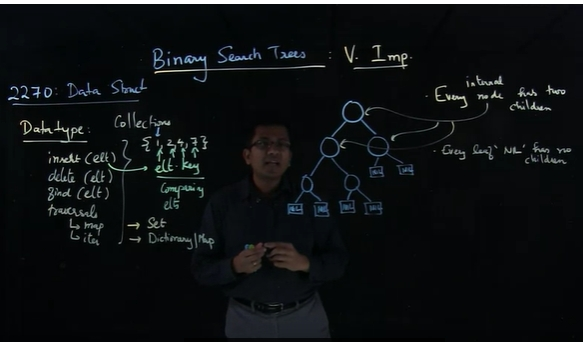
\includegraphics[width=\textwidth]{binarysearchtreenodes.png}
\end{figure}

\paragraph{
    When there is a node with the key 25, every node in the left subtree
    will have a key $<$ 25, and every node in the right subtree will
    have a key $>$ 25.\\
    The rule will also apply to all those subtrees.\\
}

\begin{figure}[H]
    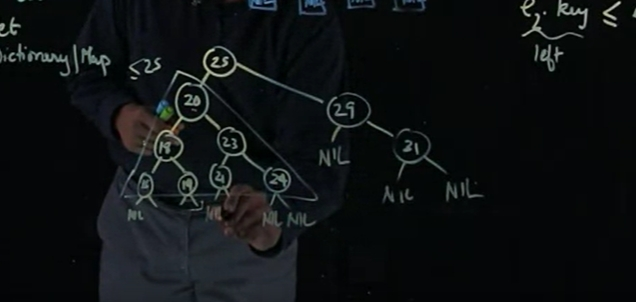
\includegraphics[width=\textwidth]{binarysearchtreerealexample.png}
\end{figure}

\begin{verbatim}
    Example:
     25
    /  \
   15  50
  / \  / \
 10 22 35 70
\end{verbatim}

\begin{verbatim}

Question:
Binary Search Trees may look similar to Heaps, but it is important 
to consider their differences.
In a Min-Heap, the smallest element must be the root node of the tree.
In a Binary Search Tree, on the other hand, how would we find the 
smallest element?

A: We would traverse the left subtree of the root node until we 
reach a leaf node, which means a node with a NIL as its left child.
\end{verbatim}

TBC at 9:09

\end{document}